\clearpage
\phantomsection
%\addcontentsline{toc}{chapter}{مقدمات}
\chapter{تعریف مساله}
\markboth{تعریف مساله}{عنوان فصل}

\section{پیاده سازی روش یادگیری خودنظارتی بر روی شبکه های عصبی ‌اسپایکی}


در این پروژه، قصد داریم از روش یادگیری متضاد ساده استفاده کنیم تا با ترکیب شبکه‌های عصبی اسپایکی با مدل نورونی نشت کننده و ادغام آتش، یادگیری خودنظارتی را بر روی داده‌ها انجام دهیم. از طریق این یادگیری خودنظارتی، قصد داریم نمایش‌های با کیفیتی از داده‌ها استخراج کنیم که می‌توانند در وظایف مختلفی مانند دسته‌بندی استفاده شوند.

با توجه به ماهیت بیولوژیکی شبکه‌های عصبی اسپایکی و پایبند بودن آن‌ها به روش عملکرد نورون‌های واقعی و توانایی در نمایش اطلاعات پردازش شده به صورت الکتریکی و با تولید اسپایک‌ها, استفاده ا این شبکه‌ها این امکان را می‌دهد تا رفتارها و ویژگی‌هایی که در مغز و سیستم عصبی واقعی مشاهده می‌شود را به دقت بیشتری شبیه‌سازی کنیم.
از طرفی بهینه بودن شبکه‌های عصبی اسپایکی در مصرف انرژی و حافظه استفاده از این شبکه‌ها را در حوزه‌های متنوعی به خصوص حوزه‌های سخت‌افزاری نورومورفیک و رباتیک و غیره ممکن ‌می‌سازد.

از سوی دیگر مزیت‌های چشمگیر روش یادگیری خودنظارتی و بی‌نیاز شدن از داده‌های برچسب‌دار برای آموزش شبکه در پیاده‌سازی این روش, با توجه به هزینه‌بر بودن فرایند تولید برچسب و هم‌چنین کمبود داده برچسب‌دار در بسیاری از حوزه‌ها, باعث شد به پیاده‌سازی روش یادگیری خودنظارتی بر روی شبکه‌های عصبی اسپایکی بپردازیم.


به این نتیجه رسیدیم که الگوریتم یادگیری خودنظارتی را بر روی یک شبکه عصبی اسپایکی پیاده‌سازی کنیم و پس از آموزش دیدن شبکه با استفاده از روش انتقال یادگیری، شبکه آموزش دیده را بر روی داده‌های برچسب‌دار برای انجام وظایفی مانند دسته‌بندی نظارت شده آزمایش کنیم.

قبل از اعمال یادگیری خودنظارتی بر روی شبکه‌های عصبی اسپایکی، اقدام به توسعه و افزایش داده‌ها می‌کنیم. این عمل با استفاده از روش‌های افزایش داده مانند چرخش، انتقال، انعکاس و تغییر مقیاس انجام می‌شود. همانطور که در توضیحات روش یادگیری متضاد ساده گفته شده، برای پیاده‌سازی این روش باید از هر داده دو نمونه افزوده شده با یکی از تغییرات گفته شده برای ورودی شبکه تولید کنیم.

پس از انجام افزایش داده، اقدام به اعمال یادگیری خودنظارتی با روش یادگیری متضاد ساده بر روی شبکه می‌کنیم. این روش یادگیری به ما امکان می‌دهد که از معماری‌های پیچیده‌تری برای استخراج نمایندگان با کیفیت از داده‌ها استفاده کنیم. به عبارت دیگر، می‌توانیم اطلاعات کاربردی را از داده‌ها بدون نیاز به برچسب‌های دسته‌بندی شده، استخراج کنیم و از این اطلاعات برای تقویت کارایی شبکه‌های عصبی اسپایکی بهره‌برداری کنیم.

در طی فرآیند یادگیری، هر یک از نمونه‌های افزوده شده به عنوان جریان اسپایکی در گام‌های زمانی به شبکه داده می‌شود و تغییرات پتانسیل نورون‌ها و هم‌چنین آرایه اسپایک‌های خروجی هر نورون در طول زمان به عنوان خروجی شبکه در نظر گرفته می‌شود. با استفاده از توابع هزینه خودنظارتی، شبکه اسپایکی می‌آموزد که برای خروجی جفت‌های مشابه از داده, با الگوی یکسان و برای جفت‌های متفاوت , با الگویی با بیشترین تفاوت اسپایک، خروجی تولید کند.

پس از آموزش شبکه برای ساخت نمایش اسپایکی از هر داده، شبکه آموزش دیده را بر روی داده‌های برچسب‌دار با تعداد کم(۲۰٪ از حجم کل داده) از دو مجموعه MNIST و CIFAR10 منتقل می‌کنیم و میزان عملکرد شبکه را روی مساله دسته‌بندی نظارت شده بررسی می‌کنیم. مشاهده می‌شود نمایش‌های تولید شده توسط شبکه از روی داده‌های بدون برچسب، در حل مساله دسته‌بندی با داده‌های برچسب‌دار با تعداد کم، موثر است و دقت عملکرد شبکه در این مساله بیشتر می‌شود. 
در نتیجه با پیاده‌سازی روش یادگیری خودنظارتی بر روی شبکه‌های عصبی اسپایکی یک ابزار جدید و قدرتمند محاسباتی ساخته می‌شود که از یک سو هزینه برچسب‌ زدن داده را کاهش می‌دهد و نیاز به داده برچسب‌دار برای محاسبه را کم می‌کند و از سوی دیگر با توجه به مزایای شبکه‌های اسپایکی, در حوزه‌های مختلف علوم اعصاب کاربرد بسیاری دارد.

\section{پیشینه تحقیق}

با توجه به نوآورانه بودن این حوزه, تاکنون تحقیقات قبلی در زمینه‌ یادگیری خودنظارتی بر روی شبکه‌های عصبی اسپایکی کمتر متعارف بوده است و اکثر آن‌ها به طور مستقل در یکی از این دو حوزه انجام شده است. با این حال، چندین تلاش پژوهشی در این حوزه به عمل آمده است که می‌توانند به نتایج جالب و مفید منجر شوند.


در یک پژوهش در حوزه تکنولوژی نورومورفیک و شبکه‌های عصبی اسپایکی به بررسی امکانات و پیشرفت‌هایی می‌پردازد که در آن از شبکه‌های عصبی اسپایکی برای انجام وظایف پیچیده‌ای در زمینه بینایی ماشین استفاده می‌شود. این مقاله با بهره‌گیری از شبکه‌های عصبی اسپایکی در یک مسئله پیچیده مانند تخمین جریان نوری نشان می‌دهد که این نوع شبکه‌ها به کمک تصمیم‌گیری خودمتحرک توانسته‌اند عملکرد بهتری در مقایسه با شبکه‌های عصبی معمولی داشته باشند.

یکی از نکات مهم این تحقیق، تلاش برای کاهش نیاز به تطبیق زمانی در ورودی‌های این شبکه‌ها است. به این معنا که شبکه‌های عصبی اسپایکی توانسته‌اند ورودی‌هایی را طراحی کنند که بدون نیاز به اطلاعات زمانی دقیق، عملکرد خوبی در مواجهه با داده‌های پویا و بدون ساختار داشته باشند. این مسئله بسیار مهم است چرا که در بسیاری از موارد در بینایی ماشین، داده‌ها به صورت زمانی تغییر می‌کنند و این توانایی بدون نیاز به تطبیق زمانی می‌تواند عملکرد سیستم را بهبود بخشد.
در شکل \ref{fig:rel1}  ایده کلی پیاده‌سازی انجام شده قابل مشاهده است.

\begin{minipage}{\linewidth}
	\centering
	\includegraphics[width=10cm]{rel1.png}
	\captionsetup{font=small} % Adjust the font size of the caption
	\captionof{figure}{تخمین جریان نوری بر مبنای واقعه‌های خودآموز برای شبکه‌های عصبی اسپایکی عمیق. جریان واقعه به بخش‌های کوچک با تعداد یکسانی از واقعه‌ها تقسیم می‌شود، سپس به شکل مناسبی قالب‌بندی می‌شود و سپس به ترتیب به شبکه وارد می‌شود. برای هر بخش، نقشه جریان نوری پیش‌بینی می‌شود که هر واقعه ورودی را با یک بردار حرکت مرتبط می‌کند. هنگامی که تعداد کافی از واقعه‌ها پردازش شده باشد، با استفاده از تابع هزینه متضاد یک مرحله یادگیری انجام می‌شود..}
	\label{fig:rel1}
\end{minipage}




دریک تحقیق دیگر, تخمین جریان نوری براساس داده‌های واقعه‌ای با شبکه‌های عصبی اسپایکی به بررسی استفاده از دوربین‌های مبتنی بر واقعه \LTRfootnote{\lr{Event-based}} برای وظایفی مانند تشخیص حرکت با سرعت بالا و ملاحظه در محیط‌های کم نور که دوربین‌های معمولی در آن‌ها با مشکلات مواجه می‌شوند، می‌پردازد. این توانایی به دلیل داشتن وضوح زمانی بالا، دامنه پویایی بالا و مصرف انرژی پایین این دوربین‌ها امکان‌پذیر می‌شود. با این حال، روش‌های بینایی ماشین معمولی و شبکه‌های عصبی مصنوعی عمیق مناسب برای کار با خروجی‌های ناهمگام و گسسته دوربین مبتنی بر واقعه نیستند. شبکه‌های عصبی اسپایکی به عنوان شبکه‌های مناسبی برای کار با خروجی‌های دوربین مبتنی بر واقعه عمل می‌کنند، اما این شبکه‌ها به تنهایی  به دلیل پدیده ناپدید شدن اسپایک‌ها در لایه‌های عمیق عملکرد مطلوبی ندارند.

برای حل این مشکلات، در این مقاله یک مدل ارائه شده است، که یک معماری شبکه عصبی هیبریدی عمیق است که شبکه‌های عصبی معمولی را با شبکه‌های عصبی اسپایکی به صورت یکپارچه ترکیب می‌کند تا به بهترین شکل ممکن از خروجی‌های دوربین مبتنی بر واقعه برای تخمین جریان نوری بهره ببرد، در حالی که کارایی را حفظ می‌کند.
 این شبکه با یادگیری خودنظارتی ر روی یک مجموعه داده آموزش داده شده و در پیش‌بینی جریان نوری عملکرد بهتری نسبت به مدل‌های شبکه‌های عصبی معمولی دارد و همچنین کارایی محاسباتی قابل توجهی را فراهم می‌کند. در شکل \ref{fig:rel2} معماری ایده پرداخته شده در پژوهش نشان داده‌شده است.


\begin{minipage}{\linewidth}
	\centering
	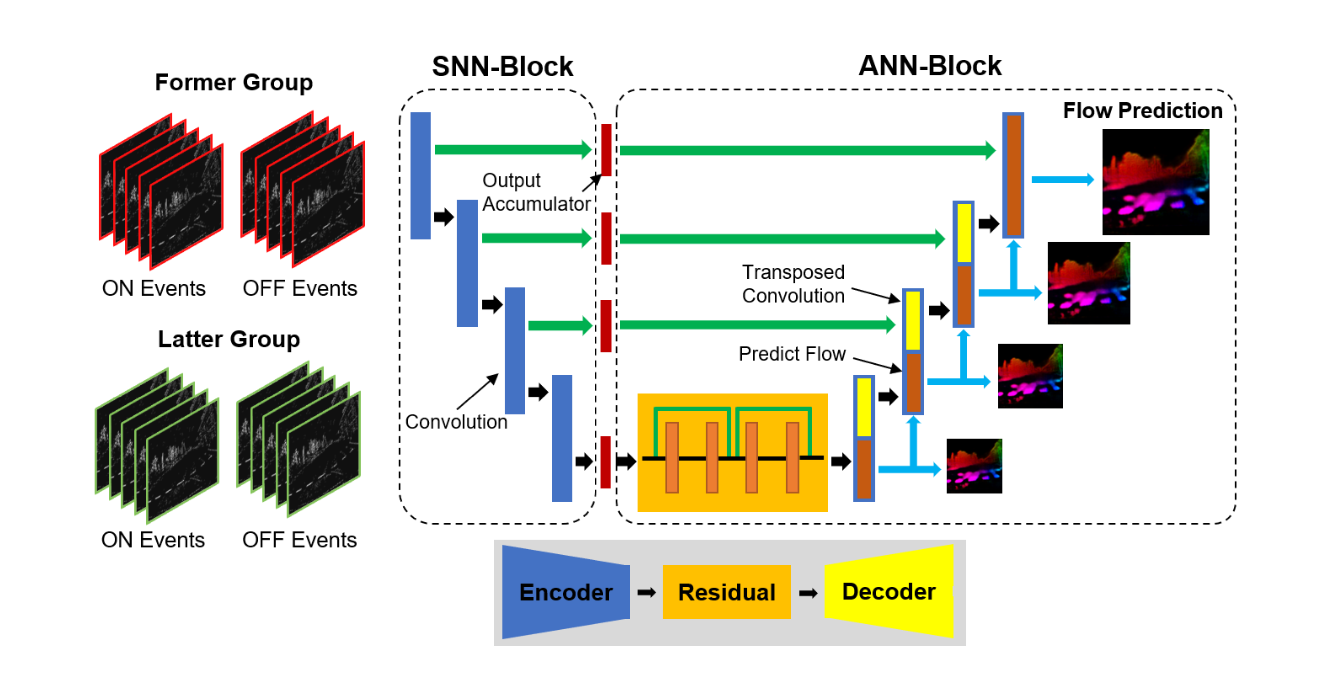
\includegraphics[width=10cm]{rel2.png}
	\captionsetup{font=small} % Adjust the font size of the caption
	\captionof{figure}{معماری شبکه ساخته شده :
		تصاویر ورودی با چهار کانال، به ترتیب از طریق شبکه هیبریدی عبور می‌کنند. بلوک اسپایکی شامل لایه‌های ورودی و سپس تجمع خروجی است، در حالی که بلوک شبکه عصبی مصنوعی شامل لایه‌های باقی‌مانده است. پس از انتقال همه چارچوب‌های واقعه ورودی پشت‌سرهم در داخل پنجره زمانی، تابع خطا ارزیابی می‌شود و روند یادگیری طی می‌شود.}
	\label{fig:rel2}
\end{minipage}





به طور کلی، تاکنون تحقیقات انجام شده در حوزه‌ یادگیری خودنظارتی بر روی شبکه‌های عصبی اسپایکی اثبات می‌کند که این روش‌ها می‌توانند به عنوان یک راهکار موثر برای بهبود عملکرد شبکه‌ها در وظایف مختلف مورد استفاده قرار گیرند. همچنین، این تحقیقات نشان می‌دهد که استفاده از دانش به‌دست‌آمده از مسائل خودنظارتی می‌تواند در تسریع یادگیری و بهبود کیفیت نمایش‌ها بسیار مؤثر باشد و پیاده‌سازی این روش‌ بر روی شبکه‌های عصبی اسپایکی با توجه به بهینه بودن و ساختار این شبکه‌ها می‌تواند در حوزه‌های مختلف بینایی ماشین نقش مهمی را ایفا کند.


\section{چالش‌ها}

چالش‌ها و مشکلاتی که در پیاده‌سازی یادگیری خودنظارتی بر روی شبکه‌های عصبی سنگین اسپایکی وجود دارند می‌توانند به شکل زیر باشند:


بالاخره، این چالش‌ها در پیاده‌سازی یادگیری خودنظارتی بر شبکه‌های عصبی سنگین اسپایکی می‌توانند به شرح زیر توضیح داده شوند:

1. نرخ اسپایک‌ها: 

در شبکه‌های عصبی اسپایکی، اطلاعات به صورت گسسته و در قالب اسپایک‌ها منتقل می‌شوند. این معمولاً به معنای این است که اطلاعاتی تنها در زمان وقوع یک اسپایک متنقل می‌شوند. بنابراین، تعیین کردن کیفیت و اهمیت این اسپایک‌ها و همچنین انتخاب زمان مناسب برای آنها می‌تواند چالش‌هایی ایجاد کند.

2. انتخاب تابع هزینه:

 انتخاب یک تابع هزینه مناسب در یادگیری خودنظارتی مهم است. این تابع باید بتواند اطلاعات مهم و قابل استفاده را از داده‌ها استخراج کند و در طی فرآیند یادگیری نمایش‌های مناسبی از داده بسازد به این صورت که نمایش‌های مربوط به یک داده افزوده شده بیشترین شباهت و با نمایش دیگر داده‌ها بیشترین تفاوت را داشته باشد. 

3. پیچیدگی محاسباتی: 

یادگیری خودنظارتی معمولاً نیازمند محاسبات پیچیده‌ای است و این محاسبات ممکن است نیاز به توانایی‌های محاسباتی قوی در سخت‌افزار داشته باشد. بنابراین، سخت‌افزارها باید مناسب برای انجام این محاسبات باشند و ممکن است فرآیند یادگیری زمان‌بر باشد.

4. دقت پایین: 

یادگیری خودنظارتی معمولاً روی داده‌های بدون برچسب انجام می‌شود و این می‌تواند به دقت پایین‌تری در مدل‌های یادگیری خودنظارتی منجر شود. این دقت پایین ممکن است چالش بزرگی را در مسائلی مانند تشخیص اشیا یا تصویربرداری از رخدادها ایجاد کند.


با توجه به نوآورانه بودن این حوزه، وجود چالش در محاسبات و پیاده‌سازی امری طبیعی است و به پشتکار و تلاش مداوم برای حاصل شدن پیشرفت نیاز دارد. در این تحقیق تلاش نموده‌ایم با پیاده‌سازی روش یادگیری خودنظارتی بر روی یک شبکه عمیق اسپایکی با چالش‌ها روبه‌رو شویم و یک نوآوری در این حوزه انجام داده و یک ابزار مفید برای انجام وظایف مختلف در حوزه یادگیری ماشین بسازیم.
